\part{The Discrete Channel with Noise}

\section{Representation of a Noisy Discrete Channel}
We now consider the case where the signal is perturbed by noise during
transmission or at one or the other of the terminals.  This means
that the received signal is not necessarily the same as that sent out
by the transmitter.  Two cases may be distinguished.  If a particular
transmitted signal always produces the same received signal, i.e., the
received signal is a definite function of the transmitted signal, then
the effect may be called distortion.  If this function has an inverse
--- no two transmitted signals producing the same received signal ---
distortion may be corrected, at least in principle, by merely performing
the inverse functional operation on the received signal.

The case of interest here is that in which the signal does not always
undergo the same change in transmission.  In this case we may assume
the received signal $E$ to be a function of the transmitted signal $S$
and a second variable, the noise $N$.
$$
E = f(S,N)
$$
The noise is considered to be a chance variable just as the message
was above.  In general it may be represented by a suitable stochastic
process.  The most general type of noisy discrete channel we shall
consider is a generalization of the finite state noise-free channel
described previously.  We assume a finite number of states and a set
of probabilities
$$
p_{\alpha,i}(\beta,j).
$$
This is the probability, if the channel is in state $\alpha$ and symbol
$i$ is transmitted, that symbol $j$ will be received and the channel left
in state $\beta$.  Thus $\alpha$ and $\beta$ range over the possible
states, $i$ over the possible transmitted signals and $j$ over the
possible received signals.  In the case where successive symbols are
independently perturbed by the noise there is only one state, and the
channel is described by the set of transition probabilities $p_i(j)$,
the probability of transmitted symbol $i$ being received as $j$.

If a noisy channel is fed by a source there are two statistical processes
at work: the source and the noise.  Thus there are a number of entropies
that can be calculated.  First there is the entropy $H(x)$ of the source
or of the input to the channel (these will be equal if the transmitter
is non-singular).  The entropy of the output of the channel, i.e.,
the received signal, will be denoted by $H(y)$.  In the noiseless case
$H(y) = H(x)$.  The joint entropy of input and output will be
$H(xy)$.  Finally there are two conditional entropies $H_x(y)$ and $H_y(x)$,
the entropy of the output when the input is known and conversely.
Among these quantities we have the relations
$$
H(x,y) = H(x) + H_x(y) = H(y) + H_y(x).
$$
All of these entropies can be measured on a per-second or a per-symbol basis.

\section{Equivocation and Channel Capacity}
If the channel is noisy it is not in general possible to reconstruct
the original message or the transmitted signal with \emph{certainty}
by any operation on the received signal $E$.  There are, however, ways
of transmitting the information which are optimal in combating noise.
This is the problem which we now consider.

Suppose there are two possible symbols 0 and 1, and we are transmitting
at a rate of 1000 symbols per second with probabilities $p_0 = p_1 =
\frac12$.  Thus our source is producing information at the rate of
1000 bits per second.  During transmission the noise introduces errors
so that, on the average, 1 in 100 is received incorrectly (a 0 as 1,
or 1 as 0).  What is the rate of transmission of information?  Certainly
less than 1000 bits per second since about 1\% of the received symbols
are incorrect.  Our first impulse might be to say the rate is 990 bits
per second, merely subtracting the expected number of errors.  This is
not satisfactory since it fails to take into account the recipient's
lack of knowledge of where the errors occur.  We may carry it to an
extreme case and suppose the noise so great that the received symbols
are entirely independent of the transmitted symbols.  The probability
of receiving 1 is $\frac12$ whatever was transmitted and similarly
for 0.  Then about half of the received symbols are correct due to chance
alone, and we would be giving the system credit for transmitting 500 bits
per second while actually no information is being transmitted at all.
Equally ``good'' transmission would be obtained by dispensing with the
channel entirely and flipping a coin at the receiving point.

Evidently the proper correction to apply to the amount of information
transmitted is the amount of this information which is missing in the
received signal, or alternatively the uncertainty when we have received a
signal of what was actually sent.  From our previous discussion of entropy
as a measure of uncertainty it seems reasonable to use the conditional
entropy of the message, knowing the received signal, as a measure of
this missing information.  This is indeed the proper definition, as we
shall see later.  Following this idea the rate of actual transmission,
$R$, would be obtained by subtracting from the rate of production (i.e.,
the entropy of the source) the average rate of conditional entropy.
$$
R = H(x) - H_y(x)
$$

The conditional entropy $H_y(x)$ will, for convenience, be called the
equivocation.  It measures the average ambiguity of the received signal.

In the example considered above, if a 0 is received the \emph{a posteriori}
probability that a 0 was transmitted is .99, and that a 1 was transmitted
is .01.  These figures are reversed if a 1 is received.
Hence
\begin{align*}
H_y(x) &= - [.99 \log .99 + 0.01 \log 0.01 ] \\
&= .081\; \text{bits/symbol}
\end{align*}
or 81 bits per second.  We may say that the system is transmitting at
a rate $1000 - 81 = 919$ bits per second.  In the extreme case where
a 0 is equally likely to be received as a 0 or 1 and similarly for 1,
the \emph{a posteriori} probabilities are $\frac12$, $\frac12$ and
\begin{align*}
H_y(x) &= - \bigl[\tfrac12\log\tfrac12+\tfrac12\log\tfrac12\bigr] \\
&= 1 \;\text{bit per symbol}
\end{align*}
or 1000 bits per second.  The rate of transmission is then 0 as it
should be.

The following theorem gives a direct intuitive interpretation of the
equivocation and also serves to justify it as the unique appropriate
measure.  We consider a communication system and an observer (or auxiliary
device) who can see both what is sent and what is recovered (with errors
due to noise).  This observer notes the errors in the recovered message
and transmits data to the receiving point over a ``correction channel''
to enable the receiver to correct the errors.  The situation is indicated
schematically in Fig.~\ref{fig:8}.
\begin{figure}[ht]
\centerline{\begin{picture}(0,0)%
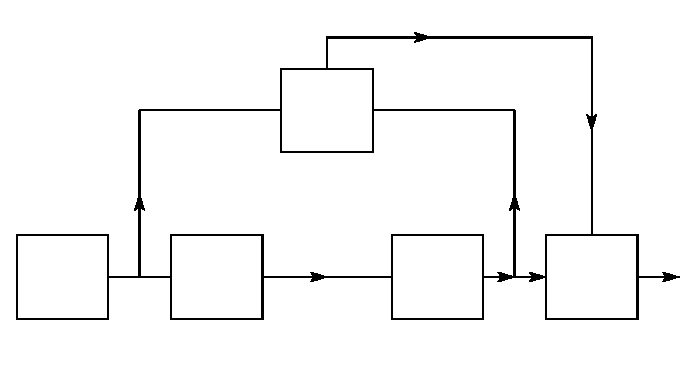
\epsfig{file=fig8.ps}%
\end{picture}%
\begin{small}%
\setlength{\unitlength}{1bp}%
\begin{picture}(318,165)
\put(22,13){\makebox(0,0){\sc source}}
\put(59,32){\makebox(0,0){\sc m}}
\put(96,13){\makebox(0,0){\sc transmitter}}
\put(202,13){\makebox(0,0){\sc receiver}}
\put(276,13){\makebox(0,0){\sc correcting}}
\put(276,5){\makebox(0,0){\sc device}}
\put(149,92){\makebox(0,0){\sc observer}}
\put(239,32){\makebox(0,0){\sc m$'$}}
\put(313,32){\makebox(0,0){\sc m}}
\put(213,163){\makebox(0,0){\sc correction data}}
\end{picture}%
\end{small}%
\endinput
}
\caption{Schematic diagram of a correction system.}
\label{fig:8}
\end{figure}

\begin{theorem}
\label{thm:10}
If the correction channel has a capacity equal to $H_y(x)$ it is possible
to so encode the correction data as to send it over this channel and
correct all but an arbitrarily small fraction $\eps$ of the errors.
This is not possible if the channel capacity is less than $H_y(x)$.
\end{theorem}

Roughly then, $H_y(x)$ is the amount of additional information that must
be supplied per second at the receiving point to correct the received
message.

To prove the first part, consider long sequences of received message $M'$
and corresponding original message $M$.  There will be logarithmically
$T H_y(x)$ of the $M$'s which could reasonably have produced each $M'$.
Thus we have $T H_y(x)$ binary digits to send each $T$ seconds.  This can
be done with $\eps$ frequency of errors on a channel of capacity $H_y(x)$.

The second part can be proved by noting, first, that for any discrete
chance variables $x$, $y$, $z$
$$
H_y(x,z) \ge H_y(x).
$$
The left-hand side can be expanded to give
\begin{gather*}
H_y(z) + H_{yz}(x) \ge H_y(x) \\
H_{yz}(x) \ge H_y(x) - H_y(z) \ge H_y(x) - H(z).
\end{gather*}
If we identify $x$ as the output of the source, $y$ as the received
signal and $z$ as the signal sent over the correction channel, then the
right-hand side is the equivocation less the rate of transmission over
the correction channel.  If the capacity of this channel is less than the
equivocation the right-hand side will be greater than zero and
$H_{yz}(x)>0$.  But this is the uncertainty of what was sent, knowing both
the received signal and the correction signal.  If this is greater than
zero the frequency of errors cannot be arbitrarily small.

\medskip\noindent{\itshape Example:}
\begin{quote}
Suppose the errors occur at random in a sequence of binary digits:
probability $p$ that a digit is wrong and $q=1-p$ that it is right.
These errors can be corrected if their position is known.  Thus the
correction channel need only send information as to these positions.
This amounts to transmitting from a source which produces binary
digits with probability $p$ for 1 (incorrect) and $q$ for 0 (correct).
This requires a channel of capacity
$$
- [p \log p + q \log q ]
$$
which is the equivocation of the original system.
\end{quote}

The rate of transmission $R$ can be written in two other forms due to
the identities noted above.  We have
\begin{align*}
R &= H(x) - H_y(x) \\
&= H(y) - H_x(y) \\
&= H(x) + H(y) - H(x,y) .
\end{align*}
The first defining expression has already been interpreted as the amount
of information sent less the uncertainty of what was sent.  The second
measures the amount received less the part of this which is due to noise.
The third is the sum of the two amounts less the joint entropy and
therefore in a sense is the number of bits per second common to the two.
Thus all three expressions have a certain intuitive significance.

The capacity $C$ of a noisy channel should be the maximum possible rate
of transmission, i.e., the rate when the source is properly matched to
the channel.  We therefore define the channel capacity by
$$
C= \max \bigl(H(x) - H_y(x)\bigr)
$$
where the maximum is with respect to all possible information sources
used as input to the channel.  If the channel is noiseless, $H_y(x) = 0$.
The definition is then equivalent to that already given for a noiseless
channel since the maximum entropy for the channel is its capacity.

\section{The Fundamental Theorem for a Discrete Channel with Noise}

It may seem surprising that we should define a definite capacity $C$
for a noisy channel since we can never send certain information in such
a case.  It is clear, however, that by sending the information in a
redundant form the probability of errors can be reduced.  For example,
by repeating the message many times and by a statistical study of the
different received versions of the message the probability of errors
could be made very small.  One would expect, however, that to make this
probability of errors approach zero, the redundancy of the encoding
must increase indefinitely, and the rate of transmission therefore
approach zero.  This is by no means true.  If it were, there would
not be a very well defined capacity, but only a capacity for a given
frequency of errors, or a given equivocation; the capacity going down as
the error requirements are made more stringent.  Actually the capacity
$C$ defined above has a very definite significance.  It is possible to
send information at the rate $C$ through the channel \emph{with as small
a frequency of errors or equivocation as desired} by proper encoding.
This statement is not true for any rate greater than $C$.  If an attempt
is made to transmit at a higher rate than $C$, say $C+R_1$, then there
will necessarily be an equivocation equal to or greater than the excess
$R_1$.  Nature takes payment by requiring just that much uncertainty,
so that we are not actually getting any more than $C$ through correctly.

The situation is indicated in Fig.~\ref{fig:9}.  The rate of information
into the channel is plotted horizontally and the equivocation vertically.
Any point above the heavy line in the shaded region can be attained and
those below cannot.  The points on the line cannot in general be attained,
but there will usually be two points on the line that can.

These results are the main justification for the definition of $C$ and
will now be proved.

\begin{theorem}
\label{thm:11}
Let a discrete channel have the capacity $C$ and a discrete source
the entropy per second $H$.  If $H \le C$ there exists a coding system
such that the output of the source can be transmitted over the channel
with an arbitrarily small frequency of errors (or an arbitrarily small
equivocation).  If $H>C$ it is possible to encode the source so that the
equivocation is less than $H-C+\eps$ where $\eps$ is arbitrarily small.
There is no method of encoding which gives an equivocation less than
$H-C$.
\end{theorem}

The method of proving the first part of this theorem is not by exhibiting
a coding method having the desired properties, but by showing that such
a code must exist in a certain group of codes.
\begin{figure}[ht]
\centerline{\begin{picture}(0,0)%
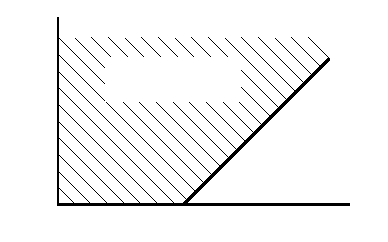
\epsfig{file=fig9.ps}
\end{picture}%
\begin{small}%
\setlength{\unitlength}{1bp}%
\begin{picture}(170,100)%
\put(75,75){\makebox(0,0){\sc attainable}}
\put(75,66){\makebox(0,0){\sc region}}
\put(80,2){\makebox(0,0){$C$}}
\put(150,2){\makebox(0,0){$H(x)$}}
\put(0,70){\makebox(0,0){$H_y(x)$}}
\put(125,45){\makebox(0,0){\rotatebox{45}{\sc slope = 1.0}}}
\end{picture}%
\end{small}%
\endinput
}
\caption{The equivocation possible for a given input entropy to a channel.}
\label{fig:9}
\end{figure}
In fact we will average the frequency of errors over this group and
show that this average can be made less than $\eps$.
If the average of a set of numbers is less than $\eps$ there must exist
at least one in the set which is less than $\eps$.  This will establish
the desired result.

The capacity $C$ of a noisy channel has been defined as
$$
C= \max\bigl(H(x) - H_y(x)\bigr)
$$
where $x$ is the input and $y$ the output.  The maximization is over
all sources which might be used as input to the channel.

Let $S_0$ be a source which achieves the maximum capacity $C$.  If this
maximum is not actually achieved by any source
let $S_0$ be a source which approximates to giving the maximum
rate.  Suppose $S_0$ is used as input to the channel.  We consider the
possible transmitted and received sequences of a long duration $T$.
The following will be true:

1. The transmitted sequences fall into two classes, a high probability
group with about $2^{T H(x)}$ members and the remaining sequences of
small total probability.

2. Similarly the received sequences have a high probability set of about
$2^{T H(y)}$ members and a low probability set of remaining sequences.

3. Each high probability output could be produced by about $2^{T H_y(x)}$
inputs.  The probability of all other cases has a small total
probability.

All the $\eps$'s and $\delta$'s implied by the words ``small'' and
``about'' in these statements approach zero as we allow $T$ to increase
and $S_0$ to approach the maximizing source.

The situation is summarized in Fig.~\ref{fig:10} where the input sequences
are points on the left and output sequences points on the right.  The
fan of cross lines represents the range of possible causes for a typical
output.

\begin{figure}[ht]
\centerline{\begin{picture}(0,0)%
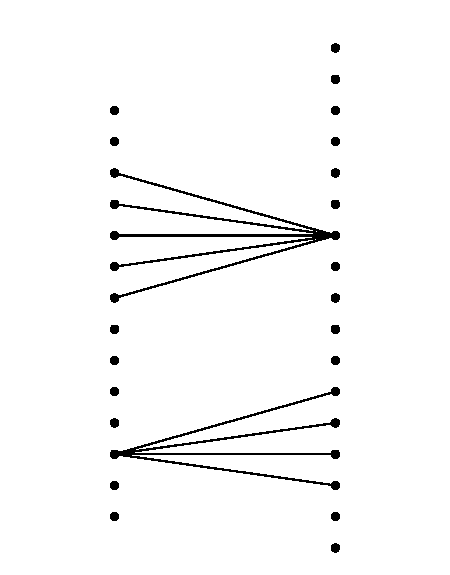
\epsfig{file=fig10.ps}
\end{picture}%
\setlength{\unitlength}{1bp}%
\begin{small}%
\begin{picture}(200,260)%
\put(47,225){\makebox(0,0){$M$}}
\put(153,255){\makebox(0,0){$E$}}
\put(0,158){\makebox(0,0)[b]{$2^{H(x)T}$}}
\put(0,150){\makebox(0,0)[b]{\sc high probability}}
\put(0,142){\makebox(0,0)[b]{\sc messages}}
\put(200,150){\makebox(0,0)[b]{$2^{H(y)T}$}}
\put(200,142){\makebox(0,0)[b]{\sc high probability}}
\put(200,134){\makebox(0,0)[b]{\sc received signals}}
\put(100,126){\makebox(0,0)[b]{$2^{H_y(x)T}$}}
\put(100,118){\makebox(0,0)[b]{\sc reasonable causes}}
\put(100,110){\makebox(0,0)[b]{\sc for each $E$}}
\put(100,28){\makebox(0,0)[b]{$2^{H_x(y)T}$}}
\put(100,20){\makebox(0,0)[b]{\sc reasonable effects}}
\put(100,12){\makebox(0,0)[b]{\sc for each $M$}}
\end{picture}%
\end{small}%
\endinput
}
\caption{Schematic representation of the relations between inputs and
outputs in a channel.}
\label{fig:10}
\end{figure}

Now suppose we have another source producing
information at rate $R$ with $R<C$.  In the period $T$ this source will
have $2^{T R}$ high probability messages.  We wish to associate these with
a selection of the possible channel inputs in such a way as to get a small frequency of errors.  We
will set up this association in all possible ways (using,
however, only the high probability group of inputs as determined by
the source $S_0$) and average the frequency of errors for this large
class of possible coding systems.  This is the same as calculating the
frequency of errors for a random association of the messages and channel
inputs of duration $T$.  Suppose a particular output $y_1$ is observed.
What is the probability of more than one message
in the set
of possible causes of $y_1$?  There are $2^{T R}$ messages distributed
at random in $2^{TH(x)}$ points.  The probability of a particular point
being a message is thus
$$
2^{T(R-H(x))}.
$$
The probability that none of the points in the fan is a message (apart
from the actual originating message) is
$$
P = \bigl[1 - 2^{T(R-H(x))}\bigr]^{2^{T H_y(x)}}.
$$
Now $R < H(x) - H_y(x)$ so $R - H(x) = - H_y(x) - \eta$ with $\eta$
positive.  Consequently
$$
P = \bigl[ 1 - 2^{-T H_y(x) - T\eta} \bigr]^{2^{T H_y(x)}}
$$
approaches (as $T\to\infty$)
$$
1-2^{-T \eta}.
$$
Hence the probability of an error approaches zero and the first part of
the theorem is proved.

The second part of the theorem is easily shown by noting that we could
merely send $C$ bits per second from the source, completely neglecting the
remainder of the information generated.  At the receiver the neglected
part gives an equivocation $H(x)-C$ and the part transmitted need
only add $\eps$.  This limit can also be attained in many other ways,
as will be shown when we consider the continuous case.

The last statement of the theorem is a simple consequence of our
definition of $C$.  Suppose we can encode a source with $H(x) = C+ a$
in such a way as to obtain an equivocation $H_y(x) = a - \eps$ with
$\eps$ positive.  Then $R=H(x)=C+a$ and
$$
H(x) - H_y(x) = C+\eps
$$
with $\eps$ positive.  This contradicts the definition of $C$ as the
maximum of $H(x) - H_y(x)$.

Actually more has been proved than was stated in the theorem.  If the
average of a set of numbers is within $\eps$ of of their maximum, a
fraction of at most $\sqrt{\eps}$ can be more than $\sqrt{\eps}$ below
the maximum.  Since $\eps$ is arbitrarily small we can say that almost
all the systems are arbitrarily close to the ideal.

\section{Discussion}

The demonstration of Theorem~\ref{thm:11}, while not a pure existence
proof, has some of the deficiencies of such proofs.  An attempt to obtain
a good approximation to ideal coding by following the method of the proof
is generally impractical.  In fact, apart from some rather trivial cases
and certain limiting situations, no explicit description of  a series of
approximation to the ideal has been found.  Probably this is no accident
but is related to the difficulty of giving an explicit construction for
a good approximation to a random sequence.

An approximation to the ideal would have the property that if the
signal is altered in a reasonable way by the noise, the original can
still be recovered.  In other words the alteration will not in general
bring it closer to another reasonable signal than the original.  This is
accomplished at the cost of a certain amount of redundancy in the coding.
The redundancy must be introduced in the proper way to combat the
particular noise structure involved.  However, any redundancy in the
source will usually help if it is utilized at the receiving point.
In particular, if the source already has a certain redundancy and
no attempt is made to eliminate it in matching to the channel, this
redundancy will help combat noise.  For example, in a noiseless telegraph
channel one could save about 50\% in time by proper encoding of the
messages.  This is not done and most of the redundancy of English remains
in the channel symbols.  This has the advantage, however, of allowing
considerable noise in the channel.  A sizable fraction of the letters
can be received incorrectly and still reconstructed by the context.
In fact this is probably not a bad approximation to the ideal in many
cases, since the statistical structure of English is rather involved and
the reasonable English sequences are not too far (in the sense required
for the theorem) from a random selection.

As in the noiseless case a delay is generally required to approach the
ideal encoding.  It now has the additional function of allowing a large
sample of noise to affect the signal before any judgment is made at the
receiving point as to the original message.  Increasing the sample size
always sharpens the possible statistical assertions.

The content of Theorem~\ref{thm:11} and its proof can be formulated in a
somewhat different way which exhibits the connection with the noiseless
case more clearly.  Consider the possible signals of duration $T$
and suppose a subset of them is selected to be used.  Let those in the
subset all be used with equal probability, and suppose the receiver is
constructed to select, as the original signal, the most probable cause
from the subset, when a perturbed signal is received.  We define $N(T,q)$
to be the maximum number of signals we can choose for the subset such
that the probability of an incorrect interpretation is less than or
equal to $q$.

\begin{theorem}
\label{thm:12}
$\displaystyle\lim_{T \to \infty}\frac{\log N(T,q)}{T} = C$, where $C$
is the channel capacity, provided that $q$ does not equal 0 or 1.
\end{theorem}

In other words, no matter how we set out limits of reliability, we can
distinguish reliably in time $T$ enough messages to correspond to about
$CT$ bits, when $T$ is sufficiently large.  Theorem~\ref{thm:12} can
be compared with the definition of the capacity of a noiseless channel
given in Section~1.

\section{Example of a Discrete Channel and its Capacity}

A simple example of a discrete channel is indicated in Fig.~\ref{fig:11}.
There are three possible symbols.  The first is never affected by noise.
The second and third each have probability $p$ of coming through
undisturbed, and $q$ of being changed into the other of the pair.
\begin{figure}[ht]
\centerline{\begin{picture}(0,0)%
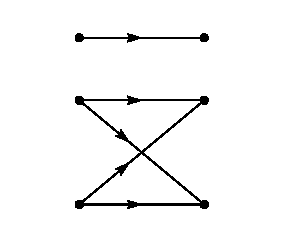
\epsfig{file=fig11.ps}
\end{picture}%
\begin{small}%
\setlength{\unitlength}{1bp}%
\begin{picture}(120,100)%
\put(60,2){\makebox(0,0){$p$}}
\put(60,67){\makebox(0,0){$p$}}
\put(40,43){\makebox(0,0){$q$}}
\put(40,25){\makebox(0,0){$q$}}
\put(0,40){\makebox(0,0){\sc transmitted}}
\put(0,32){\makebox(0,0){\sc symbols}}
\put(120,40){\makebox(0,0){\sc received}}
\put(120,32){\makebox(0,0){\sc symbols}}
\end{picture}%
\end{small}%
\endinput
}
\caption{Example of a discrete channel.}
\label{fig:11}
\end{figure}
We have (letting $\alpha = - [ p \log p + q \log q ]$ and $P$
and $Q$ be the probabilities of using the first and second symbols)
\begin{align*}
H(x) &= - P \log P - 2Q \log Q \\
H_y(x) &= 2Q \alpha.
\end{align*}
We wish to choose $P$ and $Q$ in such a way as to maximize $H(x) - H_y(x)$,
subject to the constraint $P + 2Q =1$.  Hence we consider
$$
U = - P \log P - 2Q \log Q - 2Q \alpha + \lambda (P + 2Q)
$$ 
\begin{align*}
\frac{\partial U}{\partial P} &= - 1 - \log P + \lambda = 0 \\
\frac{\partial U}{\partial Q} &= - 2 -2 \log Q - 2 \alpha + 2 \lambda = 0.
\end{align*}
Eliminating $\lambda$
\begin{align*}
\log P &= \log Q + \alpha \\
P &= Qe^{\alpha} = Q \beta 
\end{align*}
$$
P = \frac{\beta}{\beta +2} \qquad\qquad Q = \frac{1}{\beta + 2 }.
$$
The channel capacity is then
$$
C = \log \frac{\beta + 2 }{\beta}.
$$

Note how this checks the obvious values in the cases $p=1$ and $p =
\frac12$.  In the first, $\beta = 1$ and $C= \log 3$, which is correct
since the channel is then noiseless with three possible symbols.  If $p
= \frac12$, $\beta = 2$ and $C = \log 2$.  Here the second and third
symbols cannot be distinguished at all and act together like one symbol.
The first symbol is used with probability $P = \frac12$ and the second
and third together with probability $\frac12$.  This may be distributed
between them in any desired way and still achieve the maximum capacity.

For intermediate values of $p$ the channel capacity will lie between $\log
2$ and $\log 3$.  The distinction between the second and third symbols
conveys some information but not as much as in the noiseless case.
The first symbol is used somewhat more frequently than the other two
because of its freedom from noise.

\section{The Channel Capacity in Certain Special Cases}

If the noise affects successive channel symbols independently it can
be described by a set of transition probabilities $p_{ij}$.  This is
the probability, if symbol $i$ is sent, that $j$ will be received.
The maximum channel rate is then given by the maximum of
$$
-\sum_{i,j} P_i p_{ij} \log \sum_i P_i p_{ij}
	+\sum_{i,j} P_i p_{ij} \log p_{ij}
$$
where we vary the $P_i$ subject to $\sum P_i = 1$.  This leads by the
method of Lagrange to the equations,
$$
\sum_j p_{sj} \log \frac{p_{sj}}{\sum_i P_i p_{ij}} = \mu
\qquad
s = 1,2,\dots.
$$
Multiplying by $P_s$ and summing on $s$ shows that
$\mu = C$.  Let the
inverse of $p_{sj}$ (if it exists) be $h_{st}$ so that $\sum_s h_{st}
p_{sj} = \delta_{tj}$.  Then:
$$
\sum_{s,j} h_{st} p_{sj} \log p_{sj} - \log \sum_{i} P_i p_{it}
	 = C \sum_s h_{st}.
$$
Hence:
$$
\sum_i P_i p_{it} = \exp \Bigl[- C \sum_s h_{st}
	 + \sum_{s,j} h_{st} p_{sj} \log p_{sj} \Bigr]
$$
or,
$$
P_i = \sum_t h_{it} \exp \Bigl[ - C \sum_s h_{st}
	 + \sum_{s,j} h_{st} p_{sj} \log p_{sj} \Bigr].
$$

This is the system of equations for determining the maximizing values
of $P_i$, with $C$ to be determined so that $\sum P_i = 1$.  When this
is done $C$ will be the channel capacity, and the $P_i$ the proper
probabilities for the channel symbols to achieve this capacity.

If each input symbol has the same set of probabilities on the lines
emerging from it, and the same is true of each output symbol, the capacity
can be easily calculated.  Examples are shown in Fig.~\ref{fig:12}.
\begin{figure}[ht]
\centerline{\begin{picture}(0,0)%
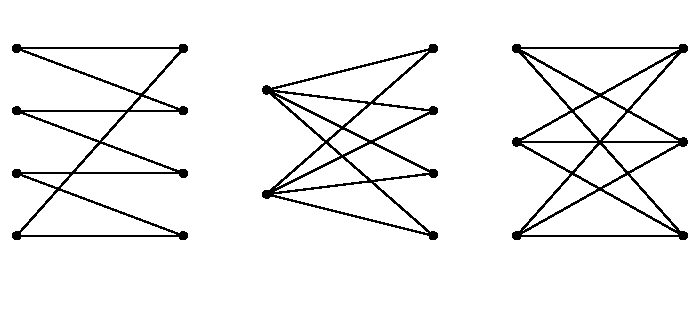
\epsfig{file=fig12.ps}
\end{picture}%
\begin{small}%
\setlength{\unitlength}{1bp}%
\begin{picture}(320,135)%
\put(40,2){\makebox(0,0){\normalsize a}}
\put(160,2){\makebox(0,0){\normalsize b}}
\put(280,2){\makebox(0,0){\normalsize c}}

\put(40,22){\makebox(0,0){\sf 1/2}}
\put(40,126){\makebox(0,0){\sf 1/2}}
\put(24,96){\makebox(0,0){\sf 1/2}}
\put(22,75){\makebox(0,0){\sf 1/2}}
\put(17,65){\makebox(0,0){\sf 1/2}}
\put(0,42){\makebox(0,0){\sf 1/2}}
\put(53,48){\makebox(0,0){\sf 1/2}}
\put(49,110){\makebox(0,0){\sf 1/2}}

\put(160,118){\makebox(0,0){\sf 1/3}}
\put(160,34){\makebox(0,0){\sf 1/3}}
\put(190,97){\makebox(0,0){\sf 1/3}}
\put(190,53){\makebox(0,0){\sf 1/3}}
\put(194,80){\makebox(0,0){\sf 1/6}}
\put(194,70){\makebox(0,0){\sf 1/6}}
\put(126,85){\makebox(0,0){\sf 1/6}}
\put(126,65){\makebox(0,0){\sf 1/6}}

\put(275,41){\makebox(0,0){\sf 1/6}}
\put(245,103){\makebox(0,0){\sf 1/6}}
\put(245,86){\makebox(0,0){\sf 1/6}}
\put(273,109){\makebox(0,0){\sf 1/3}}
\put(245,48){\makebox(0,0){\sf 1/3}}
\put(245,63){\makebox(0,0){\sf 1/3}}
\put(264,80){\makebox(0,0){\sf 1/2}}
\put(280,23){\makebox(0,0){\sf 1/2}}
\put(280,127){\makebox(0,0){\sf 1/2}}
\end{picture}%
\end{small}%
\endinput
}
\caption{Examples of discrete channels with the same transition
probabilities for each input and for each output.}
\label{fig:12}
\end{figure}
In such a case $H_x(y)$ is independent of the distribution of
probabilities on the input symbols, and is given by $-\sum p_i\log p_i$
where the $p_i$ are the values of the transition probabilities from any
input symbol.  The channel capacity is
$$
\max \bigl[ H(y) - H_x(y) \bigr] = \max H(y) + \sum p_i \log p_i.
$$
The maximum of $H(y)$ is clearly $\log m$ where $m$ is the number of
output symbols, since it is possible to make them all equally probable
by making the input symbols equally probable.  The channel capacity
is therefore
$$
C = \log m + \sum p_i \log p_i.
$$
In Fig.~\ref{fig:12}a it would be
$$
C = \log 4 - \log 2 = \log 2.
$$
This could be achieved by using only the 1st and 3d symbols.  In
Fig.~\ref{fig:12}b
\begin{align*}
C &= \log 4 - \tfrac23 \log 3 - \tfrac13 \log 6 \\
&= \log 4 - \log 3 - \tfrac13 \log 2 \\
&= \log \tfrac13 2^{\frac53}.
\end{align*}
In Fig.~\ref{fig:12}c we have
\begin{align*}
C &= \log 3 - \tfrac12 \log 2 - \tfrac13 \log 3 - \tfrac16 \log 6 \\
&= \log \frac{3}{2^{\frac12} 3^{\frac13} 6^{\frac16}}.
\end{align*}

Suppose the symbols fall into several groups such that the noise never
causes a symbol in one group to be mistaken for a symbol in another group.
Let the capacity for the $n$th group be $C_n$ (in bits per second) when
we use only the symbols in this group.  Then it is easily shown that,
for best use of the entire set, the total probability $P_n$ of all
symbols in the $n$th group should be
$$
P_n = \frac{2^{C_n}}{\sum 2^{C_n}}.
$$
Within a group the probability is distributed just as it would be if
these were the only symbols being used.  The channel capacity is
$$
C = \log \sum 2^{C_n}.
$$

\section{An Example of Efficient Coding}

The following example, although somewhat unrealistic,
is a case in which
exact matching to a noisy channel is possible.  There are two channel
symbols, 0 and 1, and the noise affects them in blocks of seven symbols.
A block of seven is either transmitted without error, or exactly one
symbol of the seven is incorrect.  These eight possibilities are equally
likely.  We have
\begin{align*}
C &= \max \bigl[ H(y) - H_x(y) \bigr] \\
&= \tfrac17 \bigl[ 7 + \tfrac88\log \tfrac18 \bigr] \\
&= \tfrac47 \;\text{bits/symbol}.
\end{align*}
An efficient code, allowing complete correction of errors and transmitting
at the rate $C$, is the following (found by a method due to R. Hamming):

Let a block of seven symbols be $X_1, X_2,\dots, X_7$.  Of these $X_3$,
$X_5$, $X_6$ and $X_7$ are message symbols and chosen arbitrarily by
the source.  The other three are redundant and calculated as follows:
$$
\begin{array}{c c@{~}c@{~}c@{~}c l c}
X_4 & \text{is} & \text{chosen} & \text{to} & \text{make}
	 & \alpha = X_4 + X_5 + X_6 + X_7 & \text{even} \\
X_2 & \text{``} & \text{``} & \text{``} & \text{``}
	 & \beta = X_2 + X_3 + X_6 + X_7 & \text{``} \\
X_1 & \text{``} & \text{``} & \text{``} & \text{``}
	& \gamma = X_1 + X_3 + X_5 + X_7 & \text{``}
\end{array}
$$
When a block of seven is received $\alpha , \beta$ and $\gamma$ are
calculated and if even called zero, if odd called one.  The binary
number $\alpha\,\beta\,\gamma$ then gives the subscript of the $X_i$
that is incorrect (if 0 there was no error).

